\documentclass[output=paper,colorlinks,citecolor=brown]{langscibook}
\author{Ekkehard König\affiliation{Free University of Berlin}\orcid{}}
\title{Beyond exophoric and endophoric uses: Additional discourse functions of demonstratives}
\abstract{It is a well-known fact that demonstratives develop endophoric uses, i.e. anaphoric and cataphoric ones, as extensions of their basic exophoric (gestural) use. In these endophoric uses the relevant expressions relate retrospectively either to a part of the preceding, or prospectively to a part of the following discourse. These three use types and their role in the development of grammatical markers have been analyzed in a wide variety of studies for a large number of languages. Far less attention has been given so far to the analysis and systematization of additional discourse functions of demonstratives, in which they have either lost the deictic or the ontological component of their meaning, or even both. The present paper analyzes such uses for a small subset of European languages, drawing a distinction between four types: (i) coordination of contrasting terms and their use to express quantification and vagueness, (ii) idiomatic combinations of basic demonstratives and their use as discourse-structuring devices, (iii) the use of demonstratives relating to evaluative rather than standard points of orientation and (iv) the basically anaphoric use of demonstratives as adverbial connectives enriched in meaning by rhetorical relations. The major focus of the study are atypical demonstratives (e.g. English \textit{so, such}), expressing the ontological components of manner, quality and degree.}
\IfFileExists{../localcommands.tex}{
  \usepackage{langsci-optional}
\usepackage{langsci-gb4e}
\usepackage{langsci-lgr}

\usepackage{listings}
\lstset{basicstyle=\ttfamily,tabsize=2,breaklines=true}

%added by author
% \usepackage{tipa}
\usepackage{multirow}
\graphicspath{{figures/}}
\usepackage{langsci-branding}

  
\newcommand{\sent}{\enumsentence}
\newcommand{\sents}{\eenumsentence}
\let\citeasnoun\citet

\renewcommand{\lsCoverTitleFont}[1]{\sffamily\addfontfeatures{Scale=MatchUppercase}\fontsize{44pt}{16mm}\selectfont #1}
  
  %% hyphenation points for line breaks
%% Normally, automatic hyphenation in LaTeX is very good
%% If a word is mis-hyphenated, add it to this file
%%
%% add information to TeX file before \begin{document} with:
%% %% hyphenation points for line breaks
%% Normally, automatic hyphenation in LaTeX is very good
%% If a word is mis-hyphenated, add it to this file
%%
%% add information to TeX file before \begin{document} with:
%% %% hyphenation points for line breaks
%% Normally, automatic hyphenation in LaTeX is very good
%% If a word is mis-hyphenated, add it to this file
%%
%% add information to TeX file before \begin{document} with:
%% \include{localhyphenation}
\hyphenation{
affri-ca-te
affri-ca-tes
an-no-tated
com-ple-ments
com-po-si-tio-na-li-ty
non-com-po-si-tio-na-li-ty
Gon-zá-lez
out-side
Ri-chárd
se-man-tics
STREU-SLE
Tie-de-mann
}
\hyphenation{
affri-ca-te
affri-ca-tes
an-no-tated
com-ple-ments
com-po-si-tio-na-li-ty
non-com-po-si-tio-na-li-ty
Gon-zá-lez
out-side
Ri-chárd
se-man-tics
STREU-SLE
Tie-de-mann
}
\hyphenation{
affri-ca-te
affri-ca-tes
an-no-tated
com-ple-ments
com-po-si-tio-na-li-ty
non-com-po-si-tio-na-li-ty
Gon-zá-lez
out-side
Ri-chárd
se-man-tics
STREU-SLE
Tie-de-mann
}
  \togglepaper[1]%%chapternumber
}{}

%Notes labelled "Author" to be checked by König
%Have König check the figures
%keep examples together
%avoid orphans
%repair hyphenation of hyphenated words, they spill into the margins
%How are forthcoming publications quoted? Year is given as "N.d." in the references, rather than "forthcoming", see König & Vezzosi

\begin{document}
\maketitle
\shorttitlerunninghead{Beyond exophoric and endophoric uses}

\section{Introduction}

It is generally acknowledged that in addition to their exophoric (deictic, gestural) use, demonstratives typically also have endophoric uses, which can be regarded as a first step in their further grammaticalisation. Building on some typological surveys (\citealt{Diessel1999Book,Dixon2003}) and on a variety of previous studies (\citealt{König2015}, \citeyear{König2017}; \citealt{KönigNishina2015}), the present chapter aims to identify and analyse additional discourse functions of demonstratives that have been so far neglected in cross-linguistic studies. Since the identification of relevant discourse functions requires a high degree of familiarity with the relevant languages, the data for this study will be mainly taken from four European languages (English, German, French, Italian), as representatives of languages with few deictic differentiations. Data will also partly come from Japanese, as a representative of languages with a rich system of relevant differentiations. Moreover, a subset of largely neglected and “atypical” demonstratives denoting the ontological dimensions of manner, quality and degree (MQD-demonstratives: German \textit{so}, \textit{solch}; English \textit{so}, \textit{such}; French \textit{ainsi}, \textit{tel}/\textit{pareil}, \textit{tellement}) will receive specific attention. Four major types of uses that cannot simply be subsumed under the exophoric or endophoric (i.e. anaphoric and cataphoric) use types will be distinguished; these types of uses either lost these basic deictic and/or ontological meaning or enriched their meaning in such a way that a basic anaphoric function is only marginally visible in their new use as adverbial connectives. These uses are found in (a) coordination of contrasting terms in a demonstrative paradigm, (b) idiomatic combinations of basic demonstratives, (c) a transfer of the \textit{origo} (i.e. the point of orientation) from the coordinates of the speech situation to some evaluative points, and (d) adverbial connectives derived from demonstratives. In addition to being identifiable on the basis of such formal properties, the relevant uses can also be characterised through the major changes leading to such uses: the loss of the deictic component of demonstratives leads to uses (a) and (c), whereas the loss of their ontological component is a salient feature of use (b). In (d) it is not the loss of a component but rather the contextual enrichment of the ontological component that underlies this use.

\section{Exophoric and endophoric uses}

Evidence from language learning (early acquisition), from language change (referent identified by gesture > referent identified in the preceding or following discourse), as well as from evolutionary hypotheses (“from gesture to grammar”, cf. \citealt{Arbib2012}) have led to more or less general agreement that the deictic (gestural, exophoric) use of demonstratives is basic and that endophoric (anaphoric and cataphoric) uses are derived from this basic source.\footnote{This is as good a place as any to point out that the question of which phenomena are to be included under the term “deixis” is a matter of some debate, ranging from very restrictive approaches (cf. \citealt{Kibrik2011}: 504ff.) to more encompassing ones (e.g. \citealt{Gerner2009}: 70).} The examples of adverbial and adnominal demonstratives with a basically spatial meaning in \REF{ex:koenig:1} and \REF{ex:koenig:2} illustrate these uses.

\ea\label{ex:koenig:1}
\ea {\textit{The restaurant over \textbf{there}} (+ pointing gesture) \textit{is where we want to go}. (exophoric)}\\
\ex {\textit{John has moved to Jakarta. Myself, I would not want to live \textbf{there}}. (anaphoric)}\\
\ex {\textit{\textbf{Here} is what he said}: “…” (cataphoric)}\\
\z
\z

\ea\label{ex:koenig:2}
\ea {\textit{\textbf{That}} (+ pointing gesture) \textit{book is exactly what I want}.} (exophoric)\\
\ex {\textit{He offered me some advice, but I did not want \textbf{that}}. (anaphoric)}\\
\ex {\textit{Let me tell you \textbf{this}}: “…” (cataphoric)}\\
\z
\z

These examples show that it is basically, though not exclusively, the distal term that also manifests the anaphoric (retrospective) use, while the proximal term acquires the cataphoric (prospective), typically quotative, use. In Japanese and Finnish, languages with three term distinctions in their systems of demonstratives, it is also the speaker-proximal anaphor (Japanese \textit{koo} ‘like this, in this way’; Finnish \textit{näin} ‘like this’) which is used as a quotative marker.

Based on observations made by \citet{Tomasello1995} and \citet{Diessel2006}, attempts have been made to unify deixis and anaphora as a single system of targeting, with the target located near or far in either the speech-external (deictic) or the speech-internal (anaphoric) environment (cf. \citealt{Talmy2017}). I will not follow this move, since it neglects the parallelism in the contrast between anaphora, the retrospective identification of referents, and cataphora, the prospective identification of referents, and the difference of both from the exophoric (deictic) one.

Demonstratives are an important source for the development of a wide variety of grammatical markers and \citet{Brugmann1904} even assumed that most grammatical categories derive from such expressions. Taking the demonstratives of our focal area as an example, the following overview (\figref{fig:koenig:1}) can be given for typical exophoric and endophoric uses of MQD-demonstratives and their further developments, on the basis of (a) historical evidence and (b) semantic reconstruction (\citealt{König2015}, \citeyear{König2017}; \citealt{KönigNishina2015}; \citeauthor{KönigVezzosi} forthcoming). Detailed empirical evidence for the relevant changes in English and partly also for those in German is provided in \citet{König2017} and in \citeauthor{KönigVezzosi} (forthcoming). Analogous developments in other languages are partly reconstructed on the basis of these analyses.

% \todo[inline]{Please have a look at the Figure. Can anything be changed/improved?}
% \begin{figure}
% \includegraphics[width=\textwidth]{figures/2_Figure1.jpg}
% \caption{Exophoric and endophoric uses of MQD-demonstratives \newline (Relative marker, e.g. English \textit{such … as}; comparative, e.g. English \textit{as … as}; booster, e.g. English \textit{so good, such kindness!}, Spanish \textit{tan}; additive, e.g. English \textit{also}; coordination, e.g. English \textit{as well as}, French \textit{ainsi que}; quotative index, e.g. English \textit{so to say}, French \textit{ainsi}, German \textit{so}; approximative, e.g. English \textit{ten students or so}, Latin \textit{quasi})}
% \label{fig:koenig:1}
% \end{figure}

\begin{figure}
\scalebox{0.7}{
\begin{forest}
 for tree={
        calign=center,
        edge={->},
        fill=lightgray,
        grow'=east, % tree direction
        parent anchor=east, child anchor=west, % edge anchors
        rounded corners, draw,
        }
[(renovation)
    [exophoric
        [anaphoric
            [propositional\\(object{,} pred. complement{,} VP)
                [affirmation]
            ]
            [conditional / causal / inferential /\\manner / concessive adverbs]
            [relative marker]
            [comparative
                [consecutive
                    [booster]
                ]
            ]
            [additive
                [coordination]
            ]
        ]
        [cataphoric
            [quotative index]
        ]
        [recognitional
            [approximative
                [focus maker]
            ]
        ]
    ]
]
\end{forest}
}
\caption{Exophoric and endophoric uses of MQD-demonstratives \newline (Relative marker, e.g. English \textit{such … as}; comparative, e.g. English \textit{as … as}; booster, e.g. English \textit{so good, such kindness!}, Spanish \textit{tan}; additive, e.g. English \textit{also}; coordination, e.g. English \textit{as well as}, French \textit{ainsi que}; quotative index, e.g. English \textit{so to say}, French \textit{ainsi}, German \textit{so}; approximative, e.g. English \textit{ten students or so}, Latin \textit{quasi})}
\label{fig:koenig:1}
\end{figure}

MQD-demonstratives are an atypical subclass of demonstratives in so far as their exophoric use combined with an appropriate pointing gesture (German \textit{Ich} \textit{möchte} \textit{ein} \textit{solches} \textit{Fahrrad} ‘I would like to have a bike like this’) does not identify the referent directly, but only a type of entity instantiated by the referent (cf. \citealt{UmbachGust2014,KönigUmbach2018}). \figref{fig:koenig:1} lists some of the clearly identifiable developments of the Old English demonstrative \textit{swa} (\textit{swa} > \textit{so}; \textit{swa}{}-\textit{lic} > \textit{swelc} > \textit{such}) and the additional developments of \textit{so} which have parallels in many other languages (cf. \citealt{König2012}, \citeyear{König2015}). The examples in \REF{ex:koenig:3} illustrate some of these targets of grammaticalisation.

\ea\label{ex:koenig:3}
\ea \textit{Will John turn up}? – \textit{I think/suppose \textbf{so}}.\footnote{In Japanese it is the hearer-proximal (medial) manner demonstrative \textit{soo} (‘like that’) which is used as a propositional anaphor.} (propositional object)\\

\ex \textit{\textbf{Such} people \textbf{as} John knew did not invite him}. (relative marker)\\

\ex \textit{John is not \textbf{so} tall as Bill}. (comparative; degree marker)\\

\ex \textit{Bill is \textbf{also} attending the meeting}. (additive focus marker)\\

\ex \textit{John’s work has been published in books and journals, \textbf{as well as} in conference proceedings}. (coordinating conjunction for nominals); cf. German \textit{ebenso wie}

\ex \textit{Of the 7000 languages \textbf{or so} spoken across the globe the majority is clearly endangered}. (approximative marker)\\

\ex {Spanish/Italian} \textit{si}; Polish \textit{tak}; English \textit{yeah swa} > \textit{yes}; \textit{quite so} (marker of affirmation)\\

\ex {German \textit{so} (quotative marker)}: \textit{Die Situation ist schwierig, \textbf{so} die Kanzlerin.} ‘“The situation is difficult,” the Chancellor said.’\\ 

\ex \textit{and so on and so forth; and such} (general extender)\\
\z
\z

In contrast to their counterparts in other Germanic languages, MQD-demonstratives in English (\textit{thus}, \textit{such}, \textit{so}) have more or less lost their exophoric use. Complex expressions, separately encoding the deictic and the content dimension (\textit{like} \textit{this}, \textit{in} \textit{this} \textit{way}, \textit{therefore}), have taken over that function. Another remarkable feature of the processes of grammaticalisation described in \figref{fig:koenig:1} is the fact that these expressions do not manifest the typical co-evolution of meaning and form. Despite a great number of semantic changes there are no concomitant morphological or phonetic changes, which could be due to the stress demonstratives normally carry and the fact that there is very little morphological or phonological substance to begin with. What the relevant examples illustrate, however, is another aspect of grammaticalisation, namely de-categorisation. Grammatical markers and function words derived from MQD-demonstratives manifest an extremely high syntactic versatility and cannot easily be assigned to a specific, limited number of lexical categories.

\section{Beyond exophoric and endophoric uses}

\subsection{Introduction}



A detailed look at individual languages and cross-linguistic similarities reveals a variety of other, e.g. discourse-structuring, uses of demonstratives beyond their well-described exophoric and endophoric ones. The major challenge for their analysis is to provide a convincing systematisation and functional analysis for such uses. In the following, four such types of use will be distinguished on the basis of formal and semantic criteria, as discussed in the introduction. Let me add a few remarks as far as the semantic criteria are concerned. The basic semantic structure of demonstratives is a very simple one and comprises two semantic dimensions: (i) a deictic one, identifying a referent in terms of its distance from the centre of orientation (\textit{origo} in the sense of \citeauthor{Bühler1934}), that is, as proximal, medial or distal (in languages with a three-term distinction) or proximal vs. distal (in languages with two-term distinctions) and (ii) an ontological (content) dimension, classifying a referent in terms of such basic semantic notions as entity, object, human being, place, direction, time, manner, quality and degree, among others. \tabref{tab:koenig:1} illustrates this dual semantic structure of demonstratives, frequently also mirrored in a bi-partite morphological structure, with the help of Armenian, a language with a rich and morphologically transparent system of deictic distinctions in contrast to the impoverished systems typically found in West-European languages.

\begin{table}
\caption{System of demonstratives in Armenian}
\label{tab:koenig:1}

\begin{tabularx}{\textwidth}{XXXXX}
\lsptoprule
& {\bfseries Definiteness} & {\bfseries Entity} & {\bfseries Place} & {\bfseries Direction}\\
Proximal & ays & sa & aystegh & aystegh\\
Medial & ayd & da & aydtegh & aydtegh\\
Distal & ayn & na & ayntegh & ayntegh\\
& {\bfseries Manner} & {\bfseries Quality} & {\bfseries Degree} & {\bfseries Quantity}\\
Proximal & ayspes & ayspisi & ayschap & aysqan\\
Medial & aydpes & aydpisi & aydchap & aydqan\\
Distal & aynpes & aynpisi & aynchap & aynqan\\
\lspbottomrule
\end{tabularx}
\end{table}
\
In some of the uses distinguished in the following sections, either the exophoric (deictic) aspect or the endophoric uses derived from it have either completely disappeared or are no longer clearly visible in English, German, French and Italian. On the other hand, demonstratives may lose the ontological aspect of their meaning or be enriched in various ways by the context and give rise to a variety of adverbial connectives. The resultant semantic distinctions can then be related to several new functions on the basis of their syntactic environments and their meaning. In the following detailed discussion of these uses, I will, largely though not exclusively, use examples and data from the focal area of MQD-demonstratives.

\subsection{Coordination of contrasting terms: Loss of deictic component}

In coordination of different members of a demonstrative paradigm, the relevant expressions lose their deictic components, while keeping their content component. The relevant sentences simply imply that a situation applies to a whole spectrum of different, non-specific reference points, thus expressing both quantification and vagueness \REF{ex:koenig:4}-\REF{ex:koenig:5}.

\ea\label{ex:koenig:4}
\ea {English:} \textit{here and there}, \textit{now and then}, textit{every now and again}, \textit{this and that}, \textit{hither and thither}, \textit{so so}; \textit{such and such}; \textit{neither here nor there} ‘not important, irrelevant’\\
\ex {German:} \textit{so oder so, sowieso} ‘anyway’, \textit{es gibt solche und solche} ‘they come in all colors/kinds’; \textit{hin und her} ‘back and forth, to and fro’, \textit{dies und das} ‘this and that’; \textit{mal so, mal so} ‘this way on one occasion, that way on another’; \textit{dann und wann} ‘now and then’\\
\ex {French:} \textit{ici et là} ‘here and there’; \textit{çà et là} ‘here and there’; \textit{ça se fait comme-çi ou comme-ça} ‘you can do it like this or like that’ \\
\ex {Spanish:} \textit{si o asa} ‘like this or like that’; \textit{aquí y allí}, \textit{aquí y allá} ‘here and there’\\
\ex {Italian:} \textit{qua e là} ‘here and there’; \textit{parlare di questo e quello} ‘to speak about this and that’; \textit{così o cosà} ‘in this or that way, either way, anyway’\\
\z
\z

\ea\label{ex:koenig:5}
\ea \textit{You still find antisemitism \textbf{here and there}}.\\
\ex German: (\textit{Im Allgemeinen sind diese Leute tolerant.}) \textit{Aber, es gibt \textbf{solche und solche}}. ‘(In general people are tolerant.) But there are good people and bad people.’

\ex French (Georges Moustaki, \textit{Ma solitude}): \textit{Elle m’a suivi \textbf{çà et là}, aux quatre coins du monde}. ‘She followed me here and there, all over the world.’

\ex {[A.]} \textit{What did you do during your vacation}? – {[B.]} \textit{Oh, \textbf{this and that}}.\\
\z
\z

It is, of course, possible to use such conjunctive combinations of semantically-related demonstratives exophorically, in combination with gestures indicating different locations or instances. This is not their typical use, however, which is meant to withhold precise information.\footnote{It is worth mentioning at this point that coordination of demonstratives from different ontological domains (\textit{here} \textit{and} \textit{now}; \textit{there} \textit{and} \textit{then}; German \textit{hin} \textit{und} \textit{weg} ‘enthusiastic’) does not have the effect of erasing the deictic meaning.} Apart from their loss of the deictic component, such coordinate combinations of demonstratives may have some interesting formal properties.\footnote{The loss of the deictic component in these expressions also shows up in the fact that relevant counterparts in other languages do not derive from demonstratives (French \textit{de} \textit{temps} \textit{en} \textit{temps}, German \textit{ab} \textit{und} \textit{zu}, \textit{hin} \textit{und} \textit{wieder} ‘now and then’)}  If there is no paradigmatic contrast in the relevant system of demonstratives, one form may be used twice (cf. German \textit{so} \textit{oder} \textit{so}) or – as examples from Spanish and Italian show (Spanish \textit{asì} \textit{o} \textit{asà}; Italian \textit{così} \textit{o} \textit{cosà}) – a second term may be specifically created for these constructions. In some cases, special unexpected forms are used which manifest a certain phonological and morphological similarity (e.g. French \textit{çà} \textit{et} \textit{là}; German \textit{dann} \textit{und} \textit{wann}), thus creating a certain formal parallelism. Moreover, subtle semantic distinctions may be found in related pairs. The two French expressions \textit{ici} \textit{et} \textit{là} and \textit{çà} \textit{et} \textit{là,} which roughly correspond to English \textit{here} \textit{and} \textit{there}, in the sense of either location or direction, manifest a subtle difference in meaning, as illustrated by the representative examples in \REF{ex:koenig:6} and \REF{ex:koenig:7}.

\ea French\label{ex:koenig:6}
\ea \textit{J’ai habité \textbf{ici et là} au cours de ma vie}. \newline ‘I have lived here and there in the course of my life.’\\

\ex \textit{J’aime me promener \textbf{ici et là} le dimanche}. \newline ‘I love walking here and there on Sundays.’\\
\z
\z

\ea French \label{ex:koenig:7}
\ea \textit{Mon fils a déposé ses affaires \textbf{çà et là} dans la maison}. \newline ‘My son put his things all over our house.’\\

\ex \textit{J’ai trouvé des réponses \textbf{çà et là} dans ma mémoire}. \newline ‘I have found answers here and there in my memory.’\\
\z
\z


The difference between these minimal pairs seems to be one of identifiability, which is still possible with the first expression, but not with the second, where the motion is less orderly and more chaotic.\footnote{This observation is based on consultation with native speakers of French (Bernard Faurie and Claire Moyse).}  A similar distinction can be found between \textit{to} \textit{and} \textit{fro} vs. \textit{hither} \textit{and} \textit{thither} in English, where the old-fashioned expressions suggests more chaotic motion.

In many European languages, these binomials typically have the proximal expression in first position, but this may differ from language to language. In Japanese, a language with pervasive three-term deictic distinctions, the medial or distal member of the paradigm invariably precedes the proximal one, as illustrated by examples in \REF{ex:koenig:8}.

\ea\label{ex:koenig:8}
\textit{soko-koko} ‘here and there’; \textit{atti-kotti} ‘this way and that way, to and fro’; \textit{are-kore} ‘this and that’; \textit{sonna-konna} ‘like this and like that’; \textit{soo-koo} ‘either way, anyway’\\
\z

\subsection{Idiomatic use as discourse-structuring device: Loss of deictic and ontological components}

It is a well-known fact that demonstratives may lose their deictic meaning, and even the other, ontological, aspect of their original meaning as well, by developing into grammatical markers. The existential use of English \textit{there} is a case in point. Originally used on the basis of the general principle that existence implies “being in some location” (cf. \citealt{Lyons1967}), the local demonstrative lost both its deictic (distal) meaning and its locative meaning. Both uses, the basic locative one and the derived existential one, are visible in \REF{ex:koenig:9}.

\ea\label{ex:koenig:9}
\textit{\textbf{There} is a dog over \textbf{there}}.\\
\z
On the other hand, a demonstrative may lose only its deictic component and develop a purely lexical meaning on the basis of its ontological component. The German counterpart of the local demonstrative \textit{there} in English, namely \textit{da}, is a clear example of such a development, denoting as it does the destination of a journey, walk or motion in general, as well as an important subset of relevant destinations, namely one’s home \REF{ex:koenig:10}.

\ea German\label{ex:koenig:10}
\ea Exophoric use
\glt \textit{Das Haus, das wir suchen, ist \textbf{da} drüben}. \newline ‘The house that we are looking for is over there.’\\

\ex Non-deictic use\footnote{Note that English \textit{there} can also have this function: \textit{We} \textit{are} \textit{almost} \textit{there}.}
\glt \textit{In einer Stunde sind wir \textbf{da}}. \newline ‘We will have reached our destination in an hour.’\\

\ex Non-deictic, non-anaphoric use
\glt \textit{Karl ist nicht \textbf{da}}. \newline ‘Karl is not home.’\\
\z
\z

The use to be discussed in what follows is a more general phenomenon and shows up in a variety of frozen idioms. In the following examples the demonstratives have all lost their deictic components, and partly also their content components. They are found in short idiomatic utterances which are typically used at transition points of verbal interactions. Given that the communicative sense of such expressions cannot easily be translated into another language, I will mainly discuss examples from two genealogically close languages, namely English and German.

Before these examples are analysed in detail, a quick word on the collection of data for this analysis is required. While the examples used so far are clear instances of grammatical constructions in English, neither requiring consultation with native speakers nor any documentation by relevant corpora, the following examples are retrievable from dictionaries or usage manuals. An analysis of their use and function would ideally have to be based on relevant examples with a rich contextual embedding, but the use of such data would require far too much space\footnote{To illustrate the enormity of such a task, let me just mention that for the use of the English discourse marker \textit{well} alone there are at least ten detailed studies.} given that in corpus-based studies of such expressions only a single expression is typically discussed in detail at a time (cf. \citealt{GolatoBetz2008,BarskeGolato2010}). For reasons of space and my goal of assessing how much of their ontological, deictic, anaphoric and cataphoric meaning these uses have lost and kept, I will therefore partly rely on such detailed studies whenever they are available, but will have to use information provided by dictionaries and introspection in many other cases.

Instead of presenting relevant data in an unordered list, I will divide them into two groups depending on whether they are primarily used in introductory, initiating conversational moves \REF{ex:koenig:11} or in responsive, conclusive ones \REF{ex:koenig:12}.

\ea\label{ex:koenig:11}
\ea \textit{Now then}! \newline (introductory move, initiating, attention getter and topic change) \\

\ex \textit{Here goes}! (introduction to doing something brave, risky, foolhardy)\\

\ex \textit{Here we go}. (introductory, exhortative)\\

\ex \textit{Hi there}! (introductory, greeting)\\

\ex \textit{There you are}. \textit{There you go}. (introductory, offer, providing service)\\
\z
\z

\ea\label{ex:koenig:12}
\ea \textit{So there}! \newline (responsive, closing an argument by maintaining a decision or view)\\

\ex \textit{And that’s that}. \newline (responsive, closing an argument, terminating further discussion)\\

\ex \textit{That’s it}! (responsive, closing an argument through agreement)\\

\ex \textit{Here we go again}. \newline (responsive, comment on the recurrence of an unpleasant situation)\\

\ex \textit{Could you pass me the sugar}? – \textit{Here you go}. \newline (responsive, compliance with a request)\\

\ex \textit{There you go}. (responsive, accepting an unsatisfactory situation)\\

\ex \textit{There we were/there he was}. \newline (closing, summing up, slowing down a story)\\

\ex \textit{Now you’re talking}. (responsive, confirming the relevance of the preceding turn for an argument)\\

\ex \textit{Don’t lose them now. They are my favorite gloves}. \newline (responsive, emphatic injunction)\\

\ex \textit{There is a good boy}! (responsive, approval or encouragement)\\

\ex \textit{There, there}! (responsive, attempt to comfort someone)\\

\ex \textit{Now really}! (reprimanding)\\

\ex \textit{Come now}! ‘Don’t exaggerate!’\\
\z
\z

Whether the development of such uses of demonstratives should be regarded as an instance of grammaticalisation or instead as an instance of “pragmaticisation” is a matter of some controversial debate (cf. \citealt{Diewald2011,Wiese2011,DegandEvers-Vermeul2015}). It is true that these examples do not manifest the co-evolution between meaning and form (formal attrition + semantic bleaching, etc.) that we find in proto-typical instances of grammaticalisation, but then – as noted above – there are very few formal reductions and changes observable in the historical development of nearly all demonstratives. What the uses illustrated in \REF{ex:koenig:11} and \REF{ex:koenig:12} certainly manifest are extensions to new contexts, persistence, de-categorisation and semantic bleaching. In view of these changes I will regard the use of demonstratives in \REF{ex:koenig:11} and \REF{ex:koenig:12} also as a result of grammaticalisation, especially since a concept of grammar that excludes dialogue-structuring devices would be too restrictive (cf. \citealt[74]{DegandEvers-Vermeul2015}).

In contrast to the heterogeneous set of expressions frequently subsumed under the term “discourse markers”, the expressions under discussion manifest a general property that justifies their inclusion under a common term. As already pointed out, these expressions typically occur at transition points of a verbal interactions, i.e. at points typically involving a change of speaker, topic, or some subpart of an interaction. This characterisation classifies these utterance types in terms of a more precise discourse function, that of being responsive and possibly terminating a phase of conversational interaction or of being a first move, an initiative, in a new subpart of a verbal exchange. It is this occurrence at transition points that justifies the label “discourse-structuring devices”.\footnote{Some of the examples in \REF{ex:koenig:11} and \REF{ex:koenig:12} have also been subsumed and discussed under the term \textit{interjections.} While the use of this term may have some justification for a characterisation of the distribution of the expressions under discussion, it does not say very much about their function.} Marking the end of an exchange can also be a signal for the beginning of a new part and some of the expressions listed above can mark both the end of a part of an interaction and the beginning of a new one.\footnote{Similar extended uses of the basic manner demonstratives \textit{nii} and \textit{soo} in Estonian are described in \citet{Keevallik2005,Keevallik2010}, where these two “pro-adverbs of manner” and their counterparts in several other languages are analysed as marking transitions between conversational activities.}

The retrospective versus prospective orientation of these expressions is, of course, reminiscent of the contrast in the standard endophoric uses between anaphoric and cataphoric uses. Indeed, these orientations can be regarded as the last trace of a more basic endophoric use of demonstratives preserved in these expressions. The typical features of anaphora and cataphora, however, are no longer there. There is no referent identified via a preceding or following expression, but simply a look back or forward to some part of an interaction.

Analogous expressions with MQD-demonstratives are also found in German. One can never be sure that one will catch all the fish in a certain terminological net, but it seems that the inventory of such expressions is smaller in German than in English and is primarily based on further developments of the manner demonstrative \textit{so} \REF{ex:koenig:13}.

\ea German\label{ex:koenig:13}
\ea \textit{Ach so}. ‘O.k., I understand.’ (responsive, removing epistemic asymmetry)\\

\ex \textit{So, so}! (responsive and initiating, accepting a previous statement and its implications)\\

\ex \textit{So}! \textit{So, das wär’s für heute}! (responsive, boundary signal after an “accomplishment”) ‘Right/well/so, that’s it for today!’\\

\ex \textit{Also}! ‘Now then!’ (initiating)\\

\ex \textit{Also dann}! (responsive, conclusive)\\

\ex \textit{Na so was}! ‘Well I never!’ (responsive, comment expressing surprise) \\

\ex \textit{Na also}! (responsive, accepting a repeated attempt as a solution)\\

\ex \textit{Nun denn}. ‘Well, all right.’ (responsive, signalling reluctant agreement)\\

\ex \textit{Nun, wir wissen das nicht genau}. ‘Well, we don’t know for sure’\footnote{In \citet[450]{Jucker1993}, the function of \textit{well} is described as indicating a shift in the relevant context.} (responsive, not providing a straight answer) \\

\ex \textit{Warum willst du dahin gehen}? – \textit{Nur so}. ‘Why do you want to go there? – I simply do.’ (responsive, meant to indicate the lack of a reason for doing something)\\

\ex \textit{Plötzlich schrie er mich an. Einfach so}. ‘Suddenly he was shouting at me. Just like that.’ (initiating, indicating that somebody had no reason for doing something unusual or outrageous) 
\z
\z

In French, there seem to be fewer discourse-structuring devices derived from demonstratives, the distal demonstrative of time \textit{alors} (<  (\textit{à} +) Latin \textit{illa hora} ‘at that hour’) being the most frequent and versatile expression in this use (\textit{et alors} ‘so what?’; \textit{alors} ‘and?’; \textit{ça alors} ‘my goodness/well, really!’; \textit{merde alors} ‘holy shit’, ‘I’ll be damned’; \textit{mince alors} ‘wow/blimey/for heaven’s sake’). As shown by the English glosses in the examples above, \textit{alors} is primarily used as a responsive discourse-structuring device, but can also indicate a change of topic (cf. \citealt{DegandFagard2011}). In contrast to the distal demonstrative \textit{alors}, which derives from a demonstrative in Late Latin (\textit{à illa hora}), its proximal counterpart \textit{maintenant} has no deictic origin and is one of the rare cases which derive from a construction composed of major lexical elements, analogous to \textit{stante pede} in Latin.

To summarise, idiomatic expressions based on demonstratives may have a use as speech acts (\textit{here is to you}!; \textit{now, now}!; \textit{hi there}!), but are more typically used as discourse-structuring devices and relate to overarching purposes and intentions of speakers and goals of an argument or discourse. There are, of course, striking differences in the form and meaning of such expressions within a language and across languages, but a common feature can be seen in the discourse-structuring function of either closing or opening a sub-sequence of an argument or interaction. These functions are clearly related to the anaphoric and cataphoric uses of the relevant demonstratives, but have to be kept distinct from these more basic uses of the same expressions. The examples in \REF{ex:koenig:11} and \REF{ex:koenig:12} suggest that local and temporal demonstratives are most frequently used for such idiomatic extensions in English, whereas it is the manner demonstrative \textit{so} which typically gives rise to such discourse-structuring devices in German.

\subsection{Reference via different points of orientation: Loss of deictic component}

The characteristic feature of the third type of special (non-canonical or extended) uses of demonstratives is a transfer of the point of orientation (\textit{origo}) from the coordinates of an utterance or a point in the development of a text to some point provided by norms, expectations, evaluations, and so on, of speakers. The relevant use thus involves an additional subjective implication and can therefore also be considered as an instance of Traugott’s general tendency of semantic change from propositional to expressive meaning or, more specifically, from meanings based in the external described situation to meanings based in the internal (evaluative / perceptual / cognitive) described situation (\citealt{Traugott1982}, \citeyear{Traugott1990}). The English (partly defective) demonstrative of degree \textit{so}, which can still be used exophorically, provides particularly good illustration of this shift in the \textit{origo}, which could also be described as a loss of the standard anchoring points of a deictic dimension. Consider the examples in \REF{ex:koenig:14}.

\ea\label{ex:koenig:14}
\ea\label{ex:koenig:14a} \textit{The fish I caught yesterday was \textbf{so}} (+ gesture) \textit{long}. \newline (exophoric, gestural use)\\

\ex\label{ex:koenig:14b} \textit{Why don’t you do it like \textbf{so}} (+ gesture)? \newline (exophoric, gestural use)\\

\ex\label{ex:koenig:14c} \textit{My fish is not \textbf{so} long/as long as the one you caught}. \newline (standard of comparison)\\

\ex\label{ex:koenig:14d} \textit{Her hair always has to be just \textbf{so}}. \newline (point of orientation provided by norm)\\

\ex\label{ex:koenig:14e} \textit{You can only eat \textbf{so} much}. \newline (point of orientation provided by capacity)\\

\ex\label{ex:koenig:14f} \textit{Mrs. Jones is always \textbf{so/sooo} helpful}. \newline (point of orientation provided by expectation)\\

\ex\label{ex:koenig:14g} \textit{I am \textbf{so} taking a long nap today}. \newline (point of orientation provided by contradictory view)\\
\z
\z

In \REF{ex:koenig:14a} and \REF{ex:koenig:14b}, the point of orientation is provided by the speech situation and a pointing or mimicking gesture. This exophoric use of \textit{so}, denoting manner or degree has become marginal in present-day English, \textit{like this} and \textit{that} being typically used instead, cf. \textit{Why don’t you do it like this}? and \textit{The fish I caught yesterday was so/that long}.. The other uses of \textit{so} are not exophoric ones. The point of orientation in \REF{ex:koenig:14c} is provided by the standard of comparison in a comparative construction. In \REF{ex:koenig:14d} it is a normative one (‘as it should be’) and in \REF{ex:koenig:14e} a point is indicated that denotes general limits of a specific action, that of eating in this case. The example in \REF{ex:koenig:14f} is generally analysed as an exclamation and identifies a point surpassing a certain standard as point of orientation. Together with \textit{very}, \textit{so} is among the five most frequently used intensifiers in English and characterises a point on a scale evaluated by the speaker as high or beyond expectation (cf. \citealt{Bolinger1972}). This use as an intensifier or booster can also be found in the use of degree demonstratives in other Germanic languages, cf. German \textit{Sie ist so intelligent}! and Dutch \textit{Ze is zo intelligent}! ‘She is so intelligent!’. Finally, \REF{ex:koenig:14g} is an instance of a recent development in American English, the relevant use of \textit{so} being generally referred to as “pre-verbal use” \citep{Boulonnais2005} or as “generation-X” \textit{so} \citep{Zwicky2007}. In that use, \textit{so} invariably bears a focal stress and emphasises the truth or factuality of a statement in the context of a contradictory view. The underlying points of orientation of the first five uses of the degree adverb \textit{so} can roughly be illustrated by \figref{fig:koenig:2}, which is simply meant to indicate that different points of orientation are involved:

% \todo[inline]{Please have a look at the Figure. Can anything be changed/improved?}
% \begin{figure}
% \includegraphics[width=\textwidth]{figures/2_Figure2.jpg}
% \caption{Degree-denoting uses of \textit{so} in English}
% \label{fig:koenig:2}
% \end{figure}

\begin{figure}
 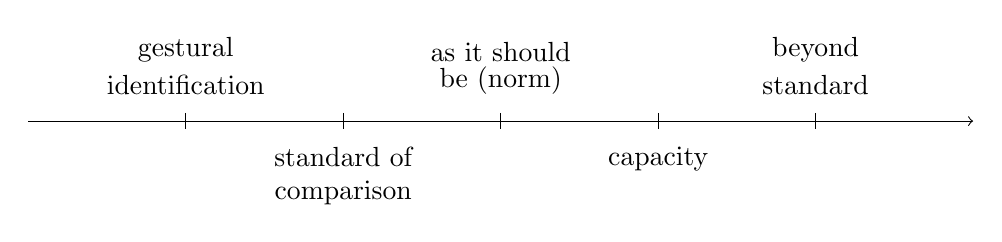
\begin{tikzpicture}
    % draw horizontal line   
    \draw[->] (0,0) -- (12,0);

    % draw vertical lines
    \foreach \x in {2,4,6,8,10}
      \draw (\x cm,3pt) -- (\x cm,-3pt);

    % draw nodes
    \draw (2,0) node[below=18pt] {} node[above=18pt] {gestural};
    \draw (2,0) node[below=6pt] {} node[above=6pt] {identification};
    \draw (4,0) node[below=6pt] {standard{ }of} node[above=6pt] {};
    \draw (4,0) node[below=18pt] {comparison} node[above=18pt] {};
    \draw (6,0) node[below=18pt] {} node[above=18pt] {as{ }it{ }should};
    \draw (6,0) node[below=6pt] {} node[above=6pt] {be{ }(norm)};
    \draw (8,0) node[below=6pt] {capacity} node[above=6pt] {};
    \draw (8,0) node[below=18pt] {} node[above=18pt] {};
    \draw (10,0) node[below=18pt] {} node[above=18pt] {beyond};
    \draw (10,0) node[below=6pt] {} node[above=6pt] {standard};
  \end{tikzpicture}
    \caption{Degree-denoting uses of \textit{so} in English}
    \label{fig:koenig:2}
\end{figure}

How can these extended uses of the demonstrative degree marker \textit{swa} (> \textit{so}) be analysed and explained? Note first of all that the last four uses are specific phenomena of English; only the exophoric uses \REF{ex:koenig:14a}-\REF{ex:koenig:14b} and the comparative endophoric use \REF{ex:koenig:14c} have clear parallels in other Germanic languages. Since an analysis of the last four uses as endophoric, i.e. as relating to a portion of preceding or following context, is excluded, a possible analysis might be to analyse them as directly deriving from the exophoric use and a shift of the \textit{origo} from the speech situation to some evaluative dimension. Extended evaluative uses of demonstratives are a widespread phenomenon, also showing up in the use of \textit{this} (‘positive’) and \textit{that} (‘negative’) in English (\textit{I like this}. vs. \textit{Oh, that}.). If such salient evaluations are frequently used in specific contexts (e.g. \textit{just}, certain types of verbs, contexts of contradicting) they can become established as being part of certain constructions.

\subsection{Connectives expressing rhetorical relations: Loss of deictic component and enrichment of meaning}

Our fourth type of non-canonical uses of demonstratives is characterised by a loss of the deictic component, combined with an enrichment, rather than a loss, of ontological meaning. Again using examples from the focal area of MQD-demonstratives, the adverbial use of English \textit{so} provides rich resources for this discussion. The examples in \REF{ex:koenig:15} illustrate the ability of English \textit{so} (< Old English \textit{swa}) to express a variety of rhetorical relations.

\ea\label{ex:koenig:15}
\ea\label{ex:koenig:15a} \textit{I did not like it. \textbf{So} I wrote to him}. (causal)\\

\ex\label{ex:koenig:15b} \textit{The whole thing was tied up in knots, \textbf{so} that we were not able to undo it.} (resultative)\\

\ex\label{ex:koenig:15c} \textit{He went into lower gear, \textbf{so} (that) his car would slow down}. (purposive)\\

\ex\label{ex:koenig:15d} \textit{He is very sick. Even \textbf{so} he goes to work}. (concessive)\\

\ex\label{ex:koenig:15e} \textit{\textbf{So} you are a linguist, eh}? - \textit{\textbf{So} what}? (inferential)\\
\z
\z

How can these uses be best characterised? Since \textit{so} does not relate to preceding utterances, but to states of affairs or propositions, the above examples are not instances of textual deixis. Their retrospective perspective certainly gives them an anaphoric character, but their semantic enrichment through the accompanying co-text clearly differentiates them from the anaphoric use as VP-anaphora and propositional anaphora found in examples like \REF{ex:koenig:16}.

\ea\label{ex:koenig:16}
\ea \textit{Bill writes his essays in the library and Mary does \textbf{so} at home}.\\
\ex A. \textit{Italy is in a very difficult situation at the moment}. – \newline B. \textit{I think/suppose \textbf{so}}.\\
\ex \textit{It might rain tomorrow. If \textbf{so} we will postpone our trip}.\\
\z
\z

Another question requiring a clear answer concerns the decision between polysemy and vagueness for the uses in \REF{ex:koenig:15}. I will opt for vagueness for the following reasons: all uses of \textit{so} in \REF{ex:koenig:15} are based on the manner reading of an anaphorically-used demonstrative. The more specific interpretation in the context of these anaphors can be derived from this manner component and the contextual information provided in the rest of the sentence. The crucial context in \REF{ex:koenig:15d} is the focus marker \textit{even}, which in combination with \textit{so}, in contrast to conditional \textit{if} (\textit{even} \textit{if} \textit{p,} \textit{q}), results in a factual, concessive interpretation. The crucial contextual information in \REF{ex:koenig:15a}-\REF{ex:koenig:15c} is the preceding factual assertion, which enriches the manner interpretation to a causal one in \REF{ex:koenig:15a} and in combination with the complementiser \textit{that} to an interpretation as consequence, either factual (resultative) or as an intention (purposive) in combination with hypothetical modality \REF{ex:koenig:15c}. Finally, it is a situational context of partial ignorance and the interrogative character of the utterance that results in the overall meaning ‘inference’ in \REF{ex:koenig:15e}.

Similar uses to \REF{ex:koenig:15} can be found for \textit{so} in German, for \textit{così} in Italian and for \textit{ainsi} in French. One of the rhetorical relations in the preceding list of examples that is notably absent in English is conditionality. The conditional use of the connective \textit{so} is somewhat archaic in Modern English and expresses a necessary condition, in contrast to the unrestricted use of German \textit{so} and French \textit{si}/\textit{ainsi} in both the protasis and the apodosis of conditionals for all types of conditionals \REF{ex:koenig:17}.

\ea\label{ex:koenig:17}
\ea {German}: \textit{\textbf{So}(fern) er rechtzeitig kommt, können wir in die Oper gehen}. ‘We can go to the opera, provided he comes in time.’\\
\ex {German}: \textit{Kommt er rechtzeitig, \textbf{so} können wir in die Oper gehen}. ‘If he comes in time we can go to the opera.’\\
\ex {German}: \textit{\textbf{So} Gott will, können wir morgen nach Italien fahren}. ‘God willing, we can go to Italy tomorrow.’ (conditional)\\
\ex {English} (OED): \textit{It is no matter how dirty a bag it is conveyed to him in, he will accept it, \textbf{so} the money is good}. (necessary condition)\\
\todo[inline]{Is OED a citation/source? How should it be integrated in the list of references?}
\ex {French} (cf. Italian \textit{se}, Spanish \textit{si}): \textit{\textbf{Si} Pierre venait aussi, (\textbf{ainsi}) nous pourrions jouer au tennis}. ‘If Pierre came too, we could play tennis together.’\\
\z
\z

It is a characteristic feature of German \textit{so} that this demonstrative combines with several adverbs, adjective and prepositions to derive subordinating conjunctions \REF{ex:koenig:18a} and adverbs \REF{ex:koenig:18b}. The relevant English counterparts of the conjunctions in German often take the form of comparative constructions.

\ea\label{ex:koenig:18} {German}\\
\ea\label{ex:koenig:18a}
 \textit{sofern} ‘providing’, \textit{sobald} ‘as soon as’, \textit{soweit}, \textit{so viel} ‘as far as’, \textit{so lange ‘as long as}’\\
\ex\label{ex:koenig:18b} \textit{sowohl} ‘both/as well’, \textit{sofort} ‘immediately’, \textit{sogleich} ‘at once’, \textit{somit} ‘consequently, therefore’, \textit{sowie} ‘as well as’,  \textit{sodann} ‘thereupon, then’\\
\z
\z

If we go beyond our focal area, English \textit{hence}, \textit{thence}, \textit{therefore}, \textit{thereby}, \textit{hereby}, \textit{but} \textit{then}, \textit{thus} also have to be included in the use type under discussion. The token-reflexive use of \textit{hereby} in combination with a performative prefix (e.g. \textit{I} \textit{hereby} \textit{declare}~…) identifies the following proposition as an explicit illocutionary act. Its distal counterpart \textit{thereby} lost its exophoric use and has a resultative meaning in a basically anaphoric use \REF{ex:koenig:19}.

\ea\label{ex:koenig:19}
\ea \textit{I \textbf{hereby} promise you never to touch hard drinks again}.\\
\ex \textit{John knocked over the red wine, \textbf{thereby} ruining the table cloth}. \\
\z
\z

Up to the time of Early Modern English, the system of demonstratives in that language also included directional demonstratives, a proximal pair (\textit{hither}, \textit{hence}) formally related to the proximal locative expression \textit{here}, and a distal pair (\textit{thither}, \textit{thence}) analogously related to the distal locative expression \textit{there}. The first member of both pairs was used to signal movement towards a goal, the location of the speaker in the case of \textit{hither} and a contextually distant location the case of \textit{thither}. The second member signalled motion away from some source, from the \textit{origo} in the case of \textit{hence} and from some contextually given place in the case of \textit{thence}. Just like most MQD-demonstratives in English, these directional uses became archaic and thus highly formal in their exophoric use (\textit{hither}) or lost that use completely (\textit{hence}). In Modern English, \textit{hence} is primarily used in an argumentative or rhetorical sense and introduces an inference based on a preceding premise \REF{ex:koenig:20}.

\ea\label{ex:koenig:20}
\textit{John got a pay rise, \textbf{hence} the new car}.\\
\z

\section{Conclusion}

Based on general typological surveys and on previous studies of MQD-demonstratives, this chapter has shown that such demonstratives have acquired a variety of additional uses as a result of losing their deictic meaning, and partly also their ontological meaning, and have developed into specific constructions, grammatical markers, or discourse-structuring devices. On the basis of data from a small subset of demonstratives, the analysis of the second type of extension beyond anaphoric and cataphoric uses was the main focus of the chapter. Four types of extended, non-canonical uses were discussed: (a) coordination of demonstratives, typically of expressions denoting the same ontological aspect but distinct deictic values, (b) short, frozen idiomatic constructions without lexical content, whose basic endophoric use is still visible in their introductory or responsive functions, (c) extended exophoric uses of the former demonstrative \textit{so} (< Old English \textit{swa}) with a shift of the centre of orientation from the speech situation to a point determined by some evaluation, and (d) basically anaphoric uses of demonstratives, metonymically enriched with meaning relating to rhetorical structure. Instead of assigning the relevant changes to a process of pragmaticisation, essentially defined as a loss of truth-conditional content, I followed the view expressed inter alia in \citet{DegandEvers-Vermeul2015} that these changes manifest crucial properties identified for grammaticalisation and can therefore be regarded as instances of such well-known changes.

It was also shown that, in English, demonstratives from several ontological dimensions have developed such extended uses as discussed above, while in German MQD-demonstratives play a prominent role in such developments. Both English and German are languages with impoverished systems of demonstratives, both in the differentiation of deictic distinctions and in the relevant ontological distinctions, but both have developed a variety of extended uses beyond the exophoric and endophoric ones. Developments of this kind, starting out from demonstratives and resulting in discourse-structuring expressions or discourse markers, are a wide-spread phenomenon. In \citet{AuerMaschler2016} it is shown that such changes starting out from the common source of proximal temporal demonstratives (\textit{nu}/\textit{nå}) are a characteristic areal feature of European languages.

\section*{Acknowledgements}

I am indebted to two anonymous reviewers, to Volker Gast and to Åshild Næss, as well as to the participants of two conferences on demonstratives (Oslo, June 14-15, 2018; Rijeka, June 28-29, 2019) for pointing out various inadequacies and suggesting possible improvements. All remaining errors are my own responsibility.

\sloppy\printbibliography[heading=subbibliography,notkeyword=this]\end{document}
